\documentclass[makesolutionspdf]{esg8022pset}
\begin{preamble}
\usepackage{amsmath}
\usepackage{amssymb}
\usepackage{enumerate}
\usepackage{graphicx}
\usepackage{hyperref}
\usepackage{mathtools}
\usepackage[per-mode=symbol]{siunitx} %If this line is giving you trouble, try replacing per-mode with per
%use inter-unit-separator={}\cdot{} ?
\providecommand{\uvec}[1]{{\hat{\bf{#1}}}}
\usepackage{pgf,tikz}
\usetikzlibrary{arrows}
\usepackage{wasysym}
\usepackage{subfig}
\makeatletter
\newcommand{\interitemtext}[1]{%
  \begin{list}{}
   {\itemindent=0mm\labelsep=0mm
   \labelwidth=0mm\leftmargin=0mm
   \addtolength{\leftmargin}{-\@totalleftmargin}}
    \item #1
  \end{list}
}
\makeatother
\renewcommand{\d}{\,d}
\providecommand{\norm}[1]{\lVert#1\rVert}

\newcommand{\Kgrad}{\left(\hat{x} \frac{\partial}{\partial x} + \hat{y} \frac{\partial}{\partial y} + \hat{z} \frac{\partial}{\partial z}\right)}
\newcommand{\Kdiv}[6]{{#4}\left(\frac{\partial {#1}}{\partial x} {#5} \frac{\partial {#2}}{\partial y} {#6}\frac{\partial #3}{\partial z} \right)}
\newcommand{\KKdiv}[6]{{#4}\left(\frac{\partial}{\partial x}{#1} {#5} \frac{\partial}{\partial y}{#2} {#6}\frac{\partial}{\partial z}{#3} \right)}
\newcommand{\dx}{\frac{\partial}{\partial x}}
\newcommand{\dy}{\frac{\partial}{\partial y}}
\newcommand{\dz}{\frac{\partial}{\partial z}}
\newcommand{\dtheta}{\frac{\partial}{\partial \theta}}
\newcommand{\dr}{\frac{\partial}{\partial r}}

\AtBeginDocument{%
  % Appologies to any future editor on the inconsistencies in TeX code and the unnecessary braces.  I'm aggregating previously typeset problems, and didn't think it worth my time to improve the quality of TeX code in ways that won't make any difference to the typeset material. -Jason Gross (jgross@mit.edu)
}%
\end{preamble}

\classname{Physics 8.022}
\semester{Spring 2011}
\problemsetnumber{10} %Put the problem set number here
\duedate{Wednesday, April 27th, 10 pm}
%\readingassignment{Kleppner and Kolenkow, \emph{An Introduction to Mechanics}, Chapters Seven and Eight}
\problemsettitle{RLC circuits, AC circuits}

\begin{document}

\begin{problem}{Purcell 7.17}
\begin{figure}[H]
    \centering
    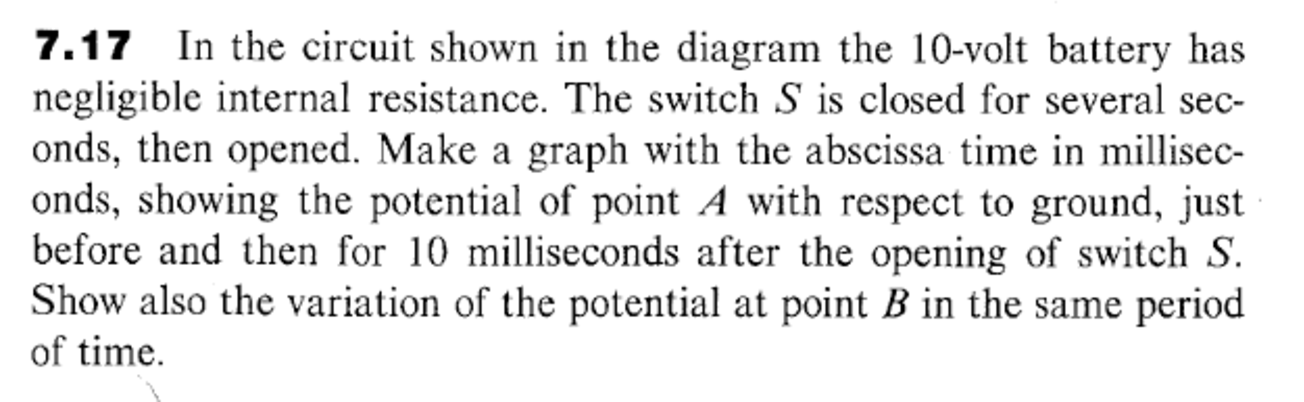
\includegraphics[width = 10cm]{pu717}
    \caption{Purcell 7.17}
  \end{figure}
  
  \begin{figure}[H]
    \centering
    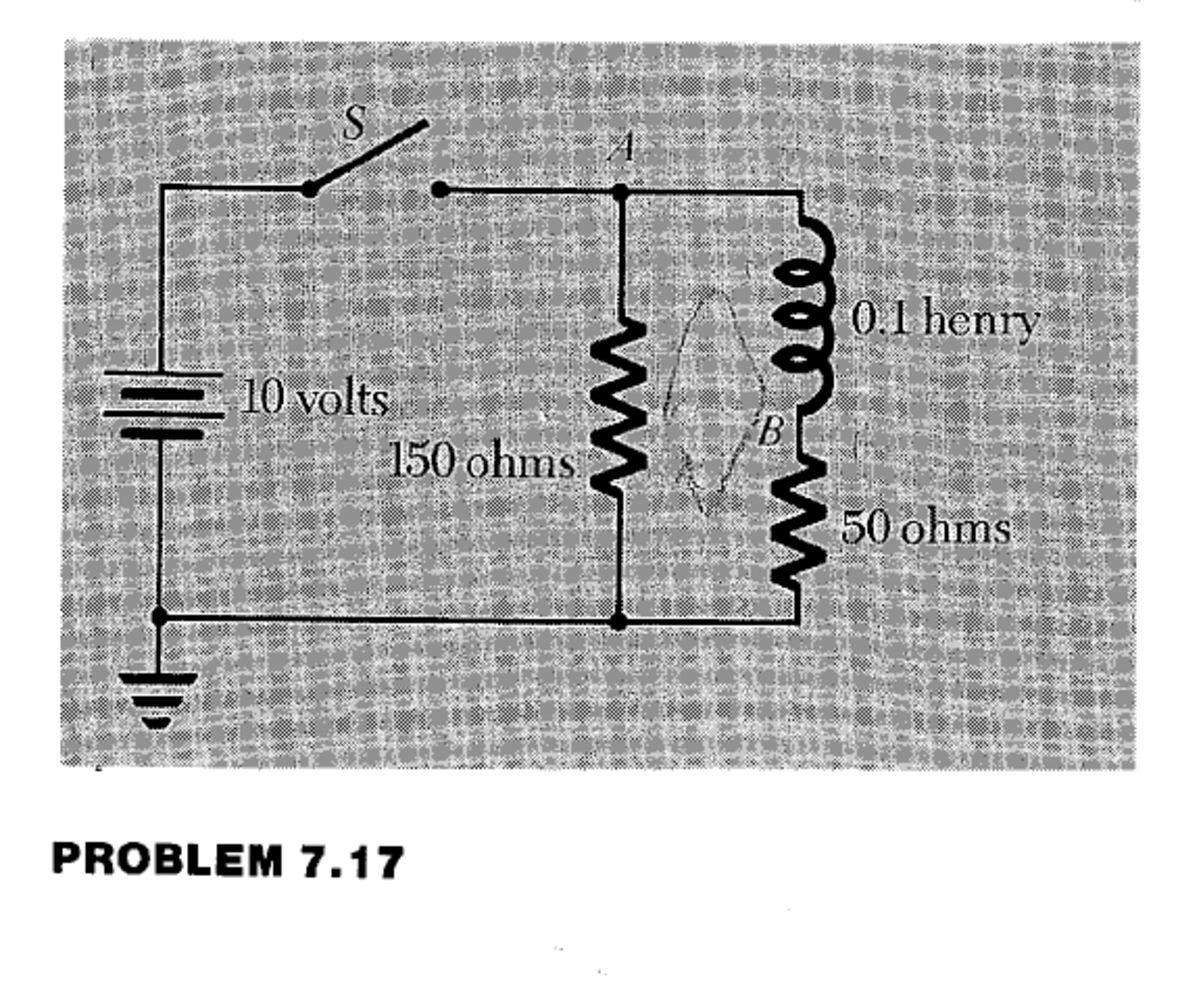
\includegraphics[width = 10cm]{figpu717}
    \caption{Figure Purcell 7.17}
  \end{figure}

 Extra question --- By grounding this circuit, we make the switch
safer to operate. Describe why a large spark jumps across the switch
when it is not grounded, and why the spark does not happen when it is
grounded.
\end{problem}
\begin{solution}


\begin{figure}[H]
    \centering
    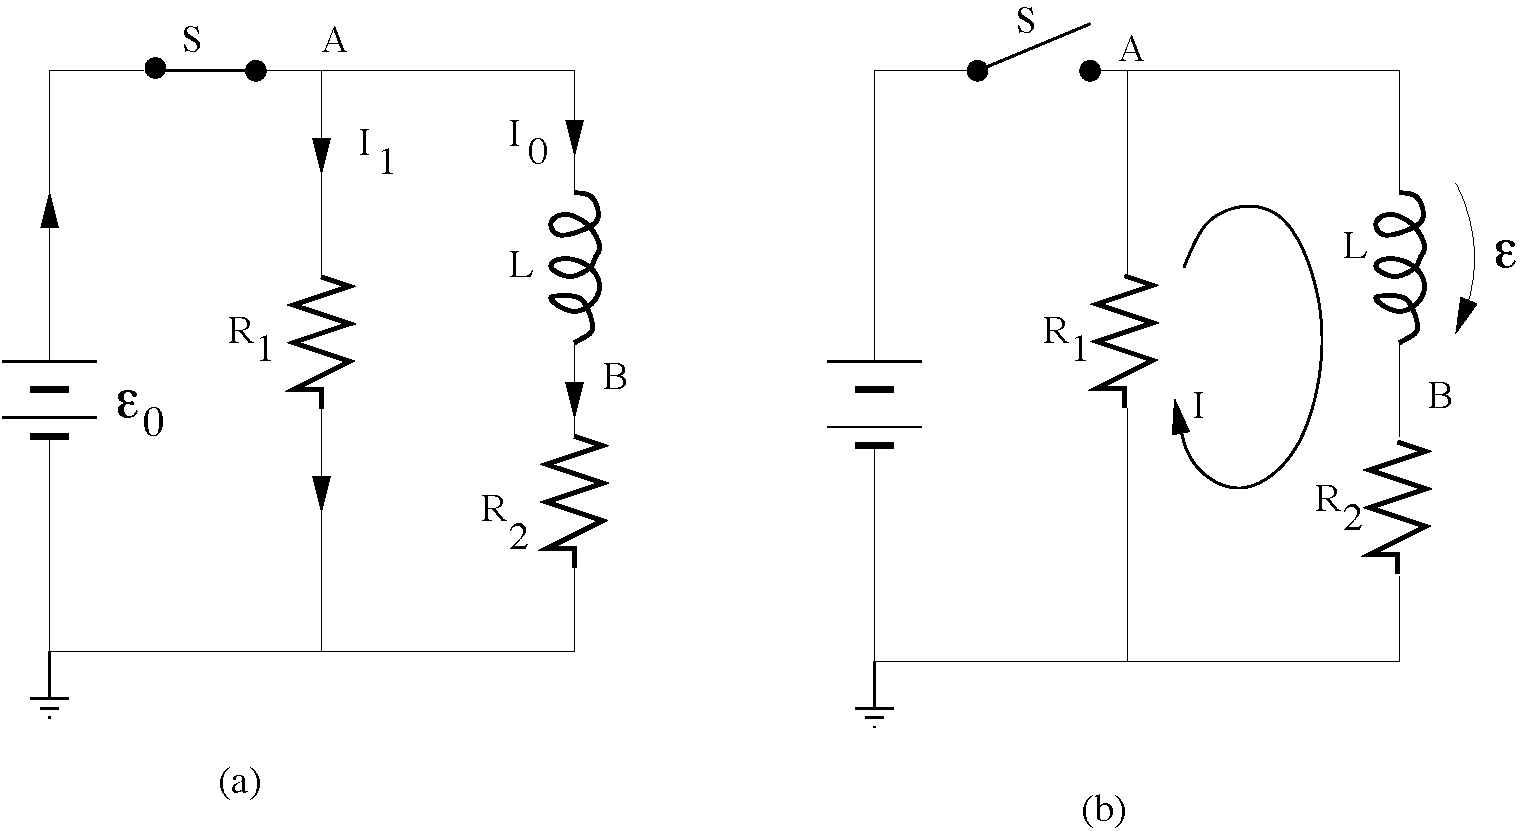
\includegraphics[width = 10cm]{inductance2}
    \caption{LR circuit: (a) steady state when switch S has been closed for a
long time; (b) the current in LR circuit when switch S is opened.}
    \label{fig:inductance2.eps}
  \end{figure}




Note: we'll use SI unit in this problem for convenience; and below
${\mathcal{E}}_0=10\:volts$, $R_1=150\:ohms$, $R_2=50\:ohms$,
$L=0.1\:henry$.\\

Switch S is closed (see Figure \ref{fig:inductance2.eps}a) for several
seconds, which is long enough that the current in the inductor is
steady; hence the EMF due to the inductor ${\mathcal{E}}=0$.  Right
right before S is opened, the current on L is $I_0 =
{\mathcal{E}}_0/R_2 = 0.2\:amp$.  The potential of point A with
respect to ground is, for $t<0$, $V_A = {\mathcal{E}}_0 = 10\:volts$;
and the potential of point B is, for $t<0$, $V_B=I_0 R_2=
{\mathcal{E}}_0=10\:volts$.\\

After switch S has been opened (Figure \ref{fig:inductance2.eps}b),
current will decay in the loop containing $L$, $R_2$ and $R_1$, and
the change in current induces an electromotive force $\mathcal{E}$ on
the inductor.  Define the positve electrmotive force and positive
current as shown in Figure \ref{fig:inductance2.eps}b; under this
convention, they satisfy ${\mathcal{E}}=-L\frac{dI}{dt}$.  Apply
Kirchhoff's rule,
\begin{equation}
-{\mathcal{E}}+I(R_1+R_2)=0.
\end{equation}
A simple calculation gives an ordinary differential equation for I:
\begin{equation}\label{eqn3:eom}
L\frac{dI}{dt}=-(R_1+R_2)I.
\end{equation}
The solution of eq.(\ref{eqn3:eom}) with initial condition
$I(t=0)=I_0$ is, for $t>0$,
\begin{eqnarray}
I(t) &=& I_0 e^{-t/\tau},\\
\textrm{where}\qquad \tau &=& L/(R_1+R_2)=0.5\: \textrm{milliseconds}.
\end{eqnarray}
The potentials of point A and point B with respect to ground are, for $t>0$
\begin{eqnarray}
V_A &=& -I(t)R_1=-I_0 R_1 e^{-t/\tau}= -30e^{-t/0.5}\;volts;\\
V_B &=& I(t)R_2=I_0 R_2 e^{-t/\tau}= 10\;e^{-t/0.5}\;volts,
\end{eqnarray}
where $t$ is in milliseconds.  The plots of potentials Vs. time are
shown in Figure \ref{fig:graph22.eps}.


\begin{figure}[H]
    \centering
    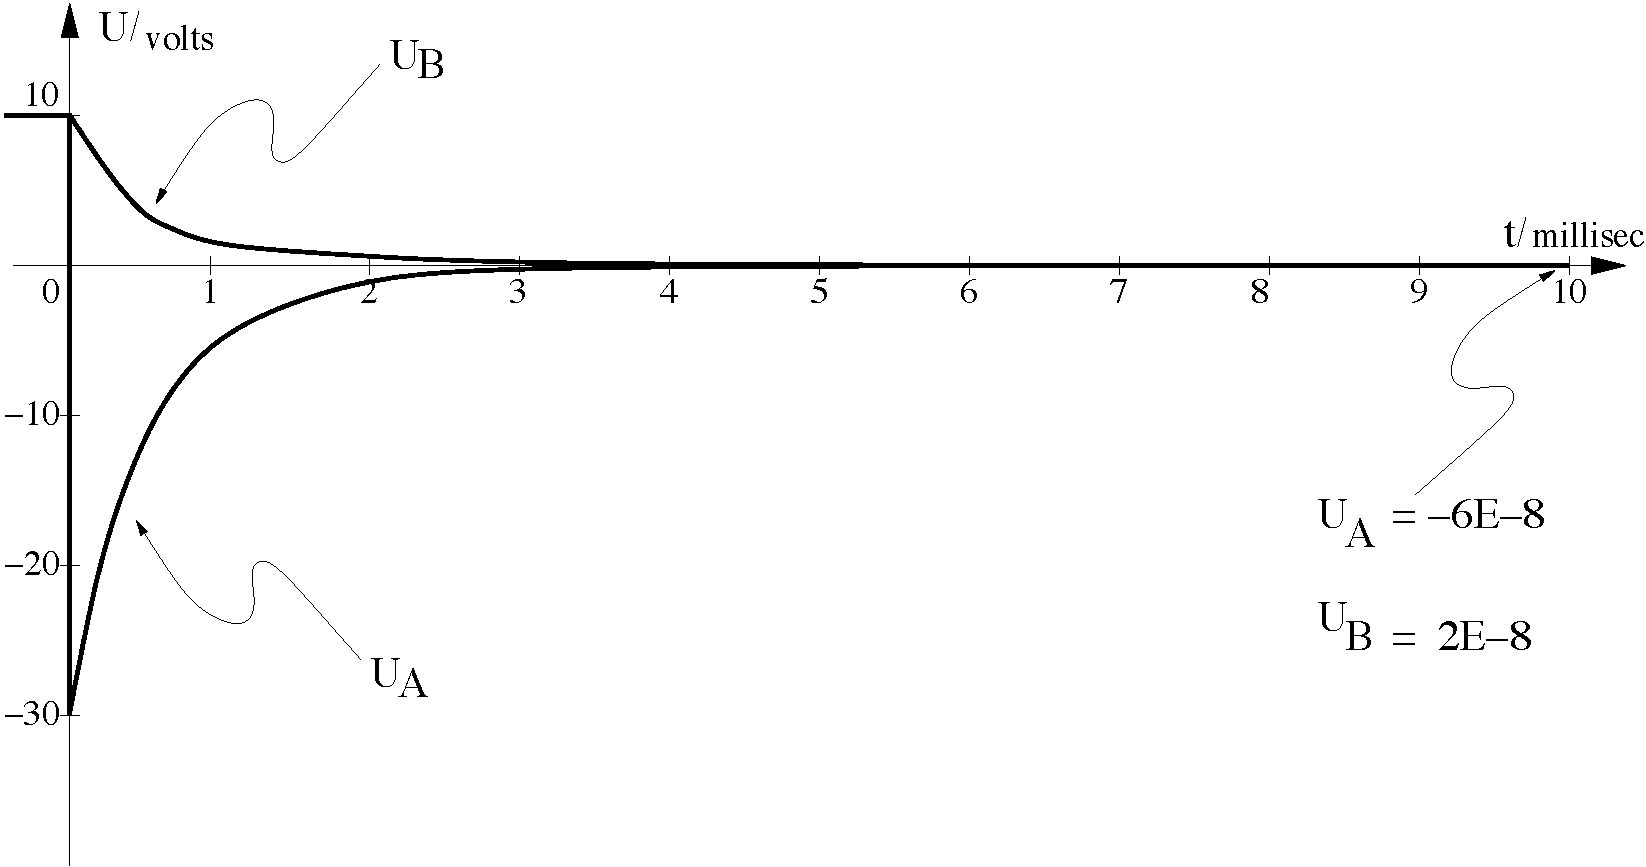
\includegraphics[width = 10cm]{graph22}
    \caption{The exponential decay of the potentials in the LR circuit.
At $t<0$, both $V_A$ and $V_B$ are at 10 volts; at $t=0$, $V_A$
abruptly drops to -30 volts, while $V_B$ is continous.}
    \label{fig:graph22.eps}
  \end{figure}


Additional question: 

Notice that the current in the 150 Ohm resistor has to abruptly switch
magnitude and direction at the moment that the switch is opened. If
the circuit were not grounded, the only way to suddenly change the
direction of the current would be to ``suck'' the current needed to
maintain continuity over from the battery -- zap!

Ground fixes this: we can think of ground as an infinite sink or
source of charge, and hence of current. By sucking (or dumping) the
current needed from ground, the current in the 150 Ohm resistor can
switch directions very rapidly -- there is no need for a big zap
across the switch.


\end{solution}

\begin{problem}{Purcell 8.4}
\begin{figure}[H]
    \centering
    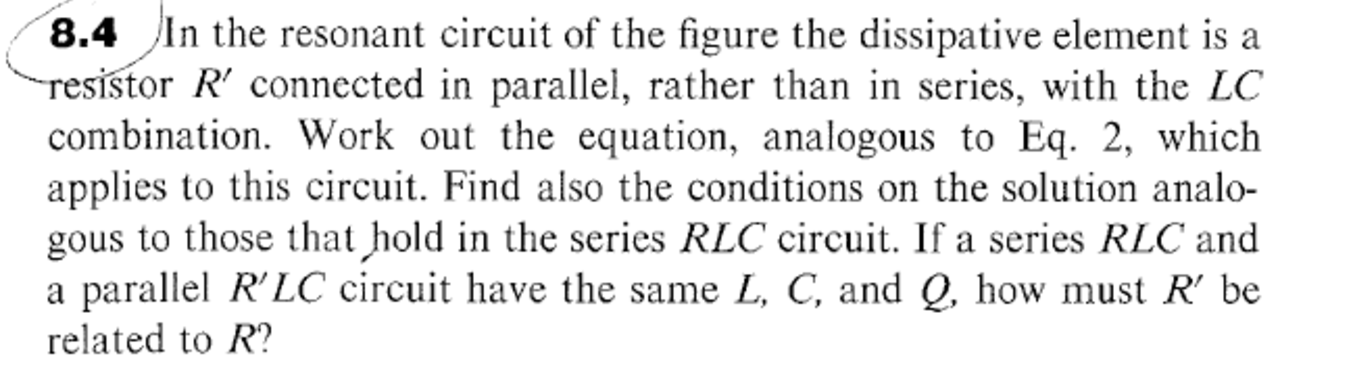
\includegraphics[width = 10cm]{pu804}
    \caption{Purcell 8.04}
  \end{figure}
  
  \begin{figure}[H]
    \centering
    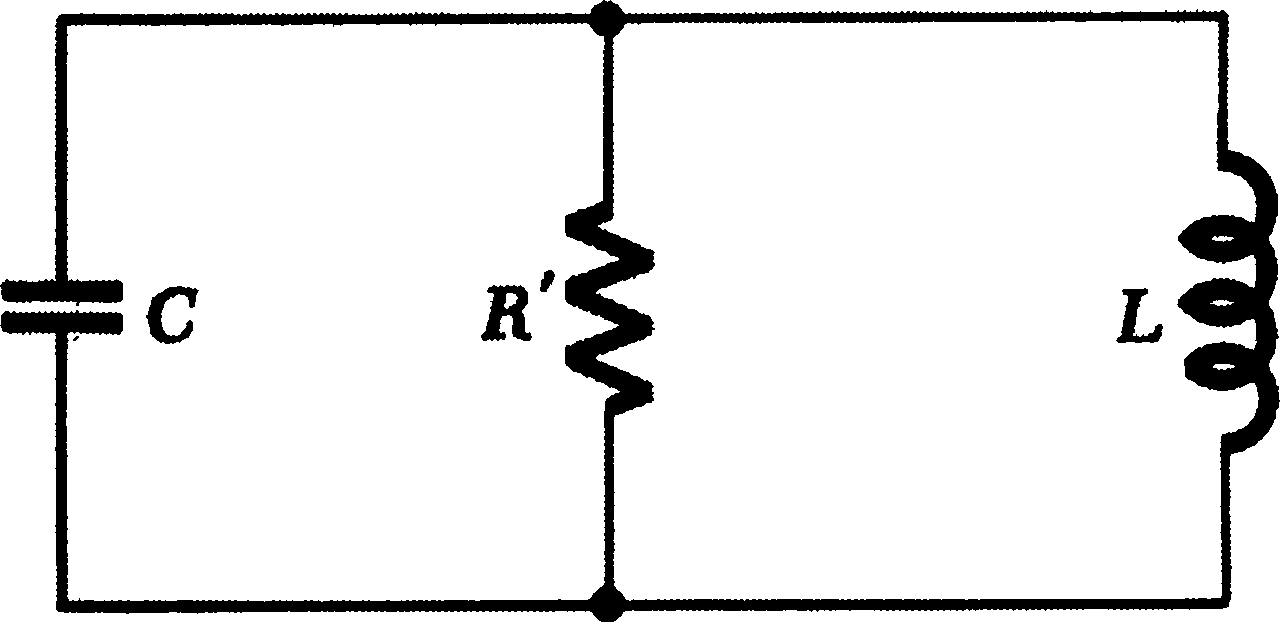
\includegraphics[width = 10cm]{figpu804}
    \caption{Purcell 8.04}
  \end{figure}
  
\end{problem}
\begin{solution}

\begin{figure}[H]
    \centering
    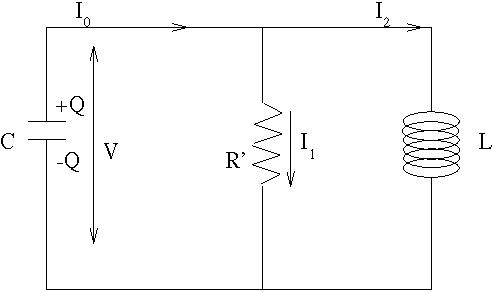
\includegraphics[width = 10cm]{ps8}
    \caption{RLC circuit}
    \label{fig:graph22.eps}
  \end{figure}


If V=Q/C is the voltage drop across the capacitor, then Kirchoff's
laws for the left and right-hand loops above give:
\begin{equation}
V-I_1R'=0
\end{equation}

\begin{equation}
-L\frac{dI_2}{dt}+I_1R'=0
\end{equation}

\begin{equation}
I_0=I_1+I_2
\end{equation}

We also know that $I_0=-dQ/dt$ and that Q=CV, so we can write
\begin{equation}
I_0=-C\frac{dV}{dt}
\end{equation}

The first Kirchoff equation gives us $I_1=V/R'$. The derivative
$dI_2/dt$ in the second equation can be written:
\begin{equation}
\frac{dI_2}{dt}=\frac{d(I_0-I_1)}{dt}=\frac{dI_0}{dt}-\frac{dI_1}{dt}=-C\frac{d^2V}{dt^2}-\frac{1}{R'}\frac{dV}{dt}
\end{equation}

Thus we can rewrite the second Kirchoff equation as a differential
equation for V:
\begin{equation}\label{eqn1:v}
\frac{d^2V}{dt^2}+\left(\frac{1}{CR'}\right)\frac{dV}{dt}+\left(\frac{1}{LC}\right)V=0
\end{equation}
Compare this to the differential equation for V in the case of a
serial LRC circuit, Purcell, Ch.8, eq.(2).
\begin{equation}\label{eqn1:v2}
\frac{d^2V}{dt^2}+\left(\frac{R}{L}\right)\frac{dV}{dt}+\left(\frac{1}{LC}\right)V=0
\end{equation}
Thus the solution to equation (\ref{eqn1:v}) can be read off directly
from the solution to equation (\ref{eqn1:v2}) (i.e. the discussion
following eq.(2) of Purcell Ch.8) by the substitution
\begin{eqnarray}
R &\rightarrow & \frac{L}{R'C}\\ \textrm{and in particular}\qquad
\alpha=\frac{R}{2L} &\rightarrow & \alpha'=\frac{1}{2R'C}
\end{eqnarray}
Analogous to the serial RLC, the oscillation frequency is real and hence
the solution oscillates when $\alpha'<\omega_0=1/\sqrt{LC}$; this
means we must have
\begin{equation}
R'>\frac{1}{2}\sqrt{\frac{L}{C}}
\end{equation}
When the parallel and serial circuits have the same L,C, and quality
factor Q (not to be confused with the charge on the capacitor), we
want to find a relation between $R'$ and $R$.  Recall that the quality
factor for the serial RLC may be written
\begin{equation}
Q=\frac{\omega}{2\alpha}=\frac{\sqrt{\omega_0^2-\alpha^2}}{2\alpha}
\end{equation}
Thus Q for the parallel RLC
\begin{equation}
Q'=\frac{\sqrt{\omega_0^2-\alpha'^2}}{2\alpha'}
\end{equation}
Clearly $Q'=Q$ implies that $\alpha'=\alpha$, or $R'=L/RC$.

\end{solution}

\begin{problem}{Purcell 8.7}
 A resonant cavity of the form illustrated is an essential part of many microwave oscillators. It can be regarded as a simple $LC$ circuit. The inductance is that of a toroid with one turn. Find an expression for the resonant frequency of this circuit and show by a sketch the configuration of the magnetic and electric fields.
 Hint: the capacitor is composed by the upper and lower disks
 \begin{figure}[H]
    \centering
    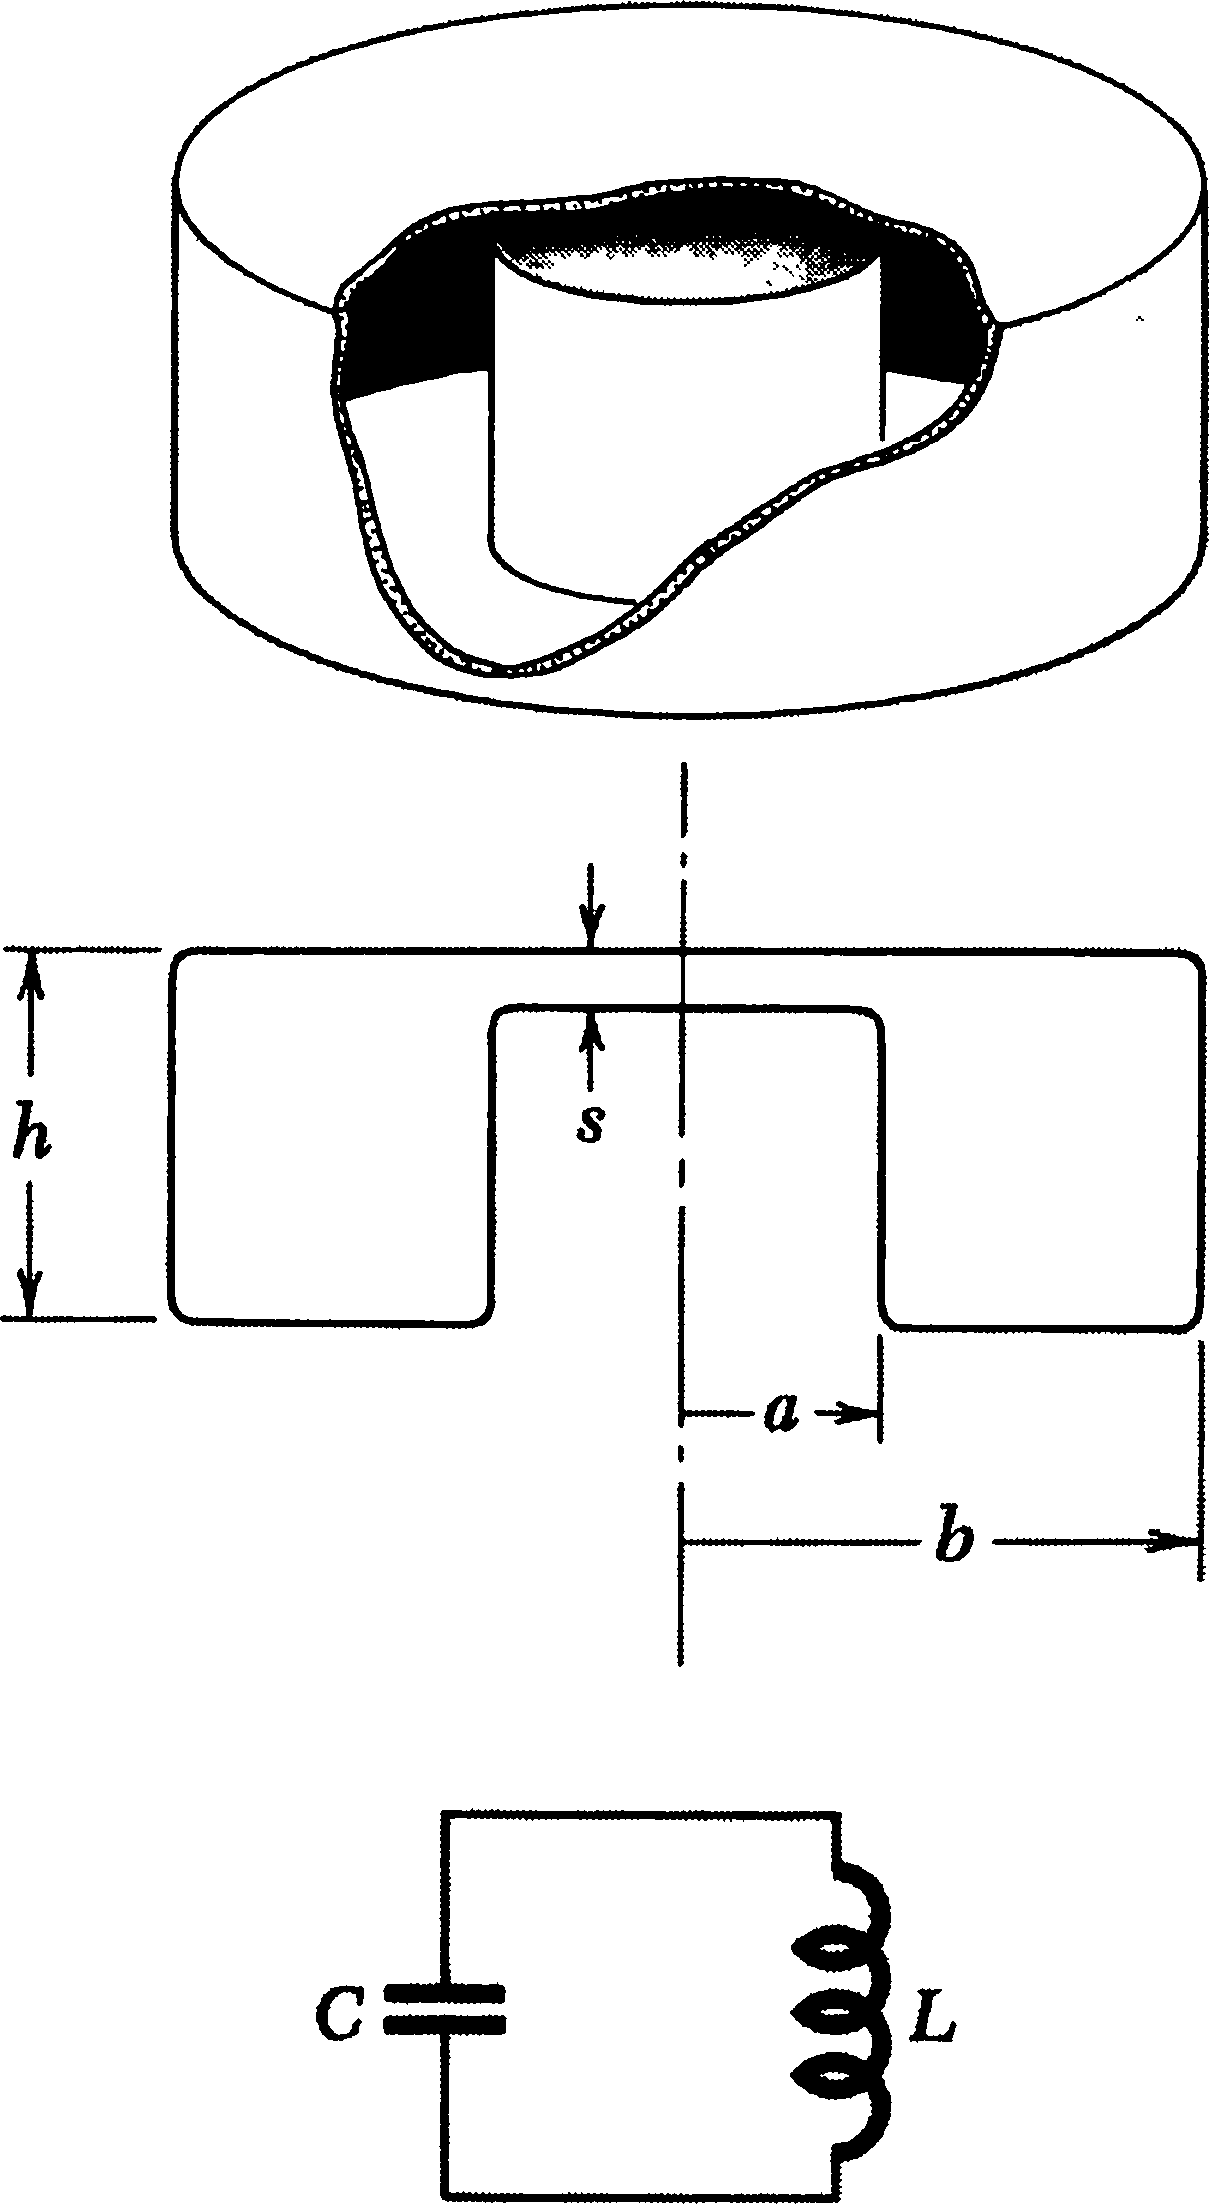
\includegraphics[width = 4cm]{pu807}
    \caption{Purcell 8.7}
    \label{fig:cavity2}
  \end{figure}
  
\end{problem}

\begin{solution}

The resonant cavity is equivalent to a simple LC circuit.  The
inductor is a configuration of currents uniformly flowing up and down 
on the surface of the inner conducting cylinder and the outer one.
The capacitor is a pair of parallel plates of seperation $s$ and area
$A=\pi a^2$.  Quote the result in Problem 8 of pset 8: the inductance
{\sl per unit length} is 
\[ L/l =\frac{2}{c^2}\ln{(\frac{b}{a})}.\]
This gives the total inductance 
\[ L= (h-s)\frac{2}{c^2}\ln{(\frac{b}{a})}.\]
[You could also use Purcell (58) of Chapter 7; you would get $h$ in place of $h-s$, which is good enough 
for small $s$.]

The capacitor is $C= A/4\pi s= a^2/4s$.  So the resonant frequency is
\begin{equation}
\omega_0=\frac{1}{\sqrt{LC}}= \left(\frac{a^2
(h-s)}{2sc^2}\ln(\frac{b}{a})\right)^{-1/2}
\approx  \left(\frac{a^2
h}{2sc^2}\ln(\frac{b}{a})\right)^{-1/2}.
\end{equation}

The configuration of the electric and magnetic field is shown in
Figure \ref{fig:cavity2}.

\begin{figure}[H]
    \centering
    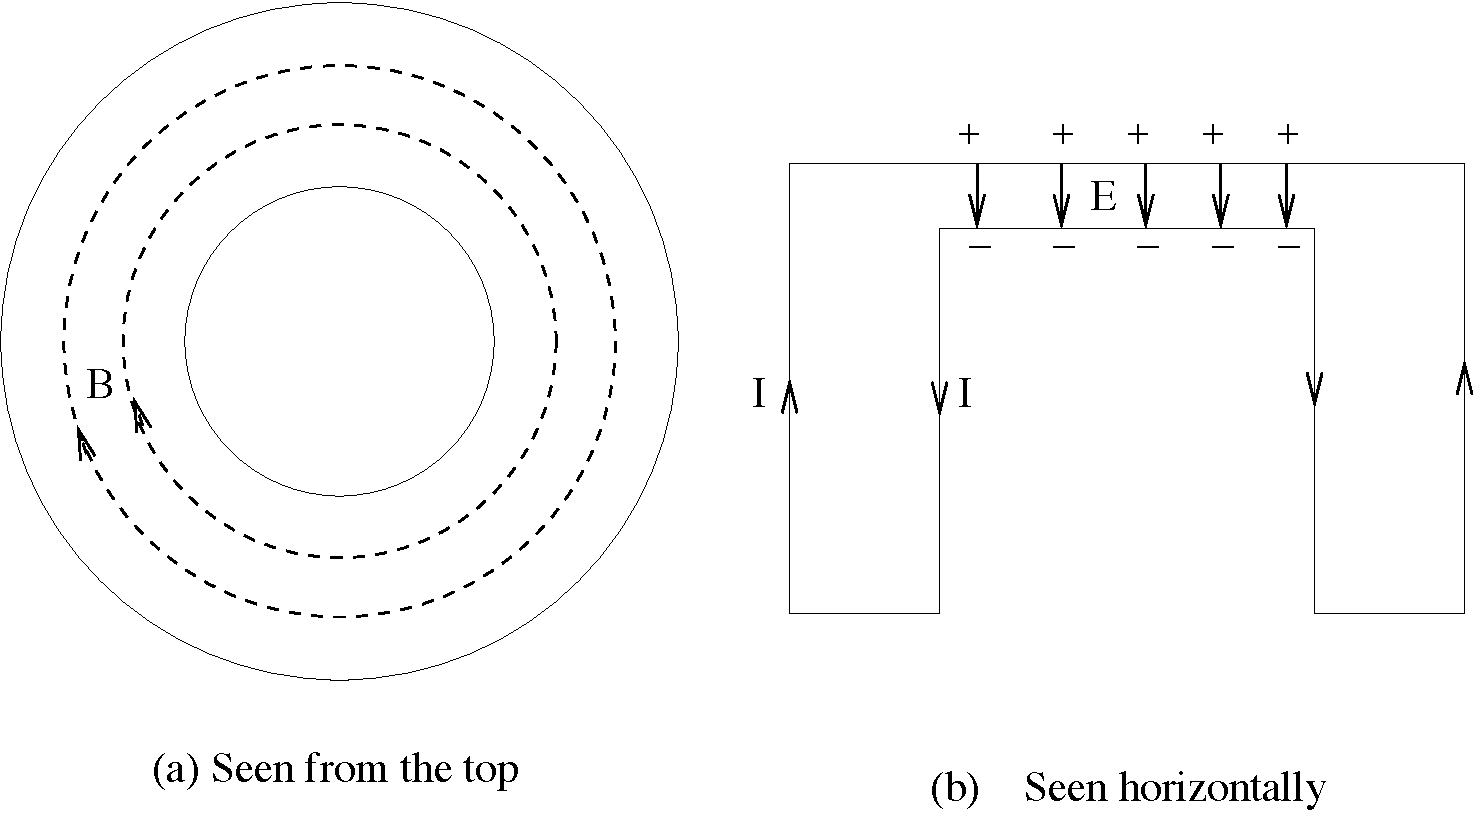
\includegraphics[width = 5cm]{cavity2}
    \caption{The configuration of $\vec{B}$ (a) and $\vec{E}$ field (b).
The magnetic field lines are circles between the inner and the outer
cylinders.  The electric field lines are parallel straight lines
between the top plates.}
    \label{fig:cavity2}
  \end{figure}


\end{solution}


\begin{problem}{Purcell 8.9}
\begin{figure}[H]
    \centering
    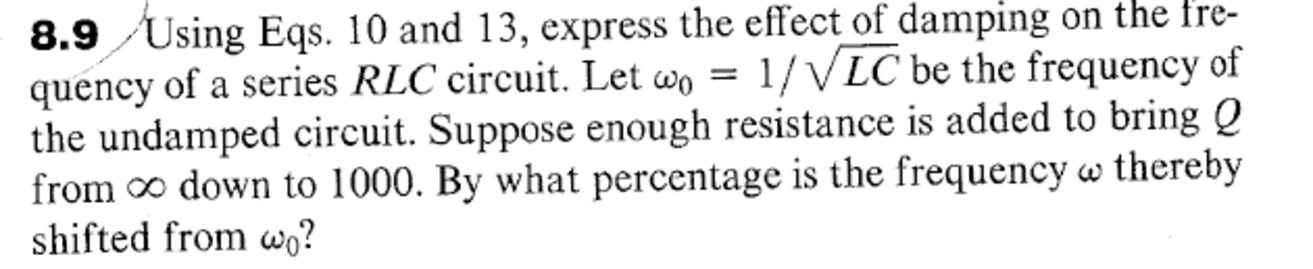
\includegraphics[width = 10cm]{pu809}
    \caption{Purcell 8.09}
  \end{figure}
  
  \begin{figure}[H]
    \centering
    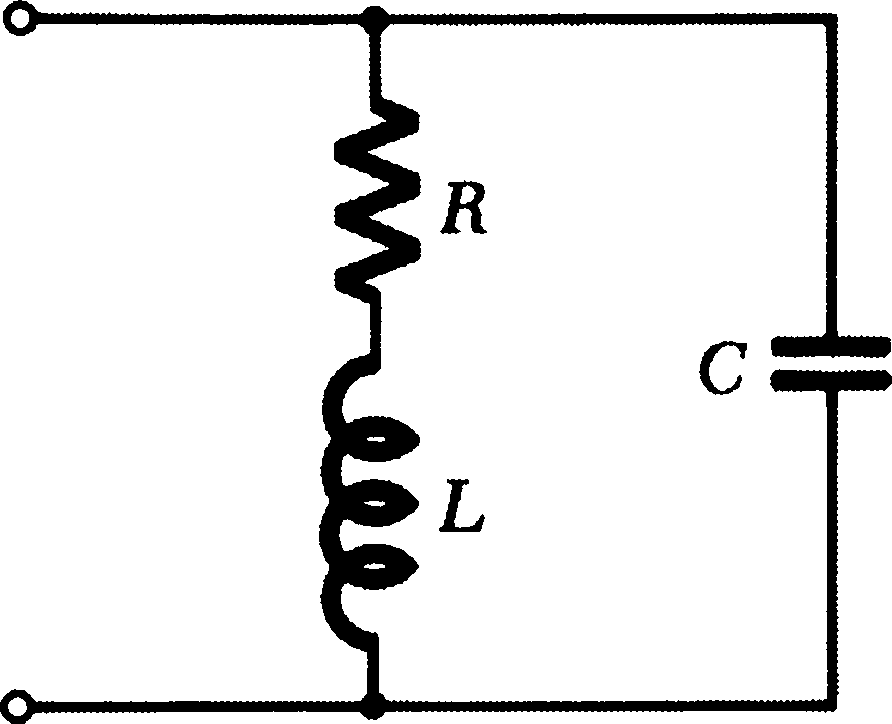
\includegraphics[width = 10cm]{figpu809}
    \caption{Purcell 8.09}
  \end{figure}
\end{problem}
\begin{solution}
Use eqs.(13) or (14) of Purcell p.301-302.
\begin{equation}
R=\frac{\omega L}{Q} \quad\to\quad \frac{R}{L}=\frac{\omega}{Q}\,.
\end{equation}
Plug this into eq.(10) of Purcell p.299.
\begin{eqnarray}
\omega^2 &=& \omega_0^2-\frac{\omega^2}{4Q^2},\\
\textrm{so} \qquad \omega &=& \omega_0 \left(1+\frac{1}{4Q^2}\right)^{-1/2}\\
&=& \omega_0\frac{2Q}{\sqrt{1+4Q^2}}.
\end{eqnarray}
where $\omega_0=1/\sqrt{LC}$.  The percentage change is
\begin{eqnarray}
\textrm{Percentage change} &=& \frac{\omega_0-\omega}{\omega_0}\times
100\%\nonumber\\
&=& \left[1-\left(1+\frac{1}{4Q^2}\right)^{-1/2}\right]\times 100\%\nonumber\\
&\approx & \frac{1}{8Q^2}\times 100\%\nonumber\\
&=& 1.25\times 10^{-5} \%,
\end{eqnarray}
for $Q=1000$.  (The binomial expansion was used to simplify the exact formula.)

\end{solution}



\begin{problem}{Purcell 8.12}

\begin{figure}[H]
    \centering
    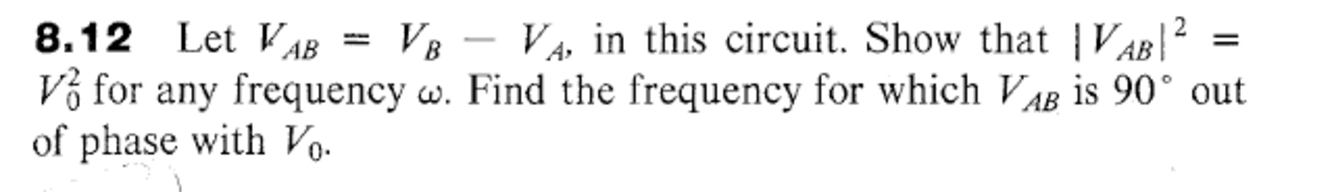
\includegraphics[width = 10cm]{pu812}
    \caption{Purcell 8.12}
  \end{figure}
  
  \begin{figure}[H]
    \centering
    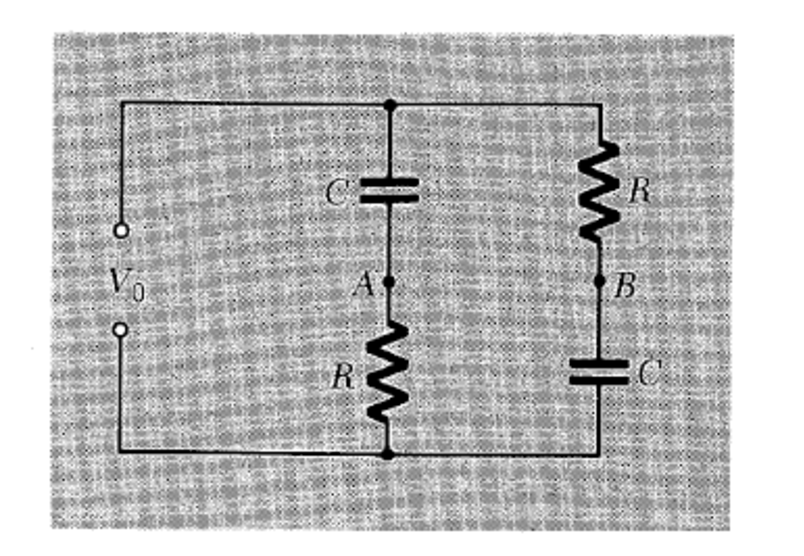
\includegraphics[width = 10cm]{figpu812}
    \caption{Purcell 8.12}
  \end{figure}
\end{problem}
\begin{solution}
\begin{figure}[H]
    \centering
    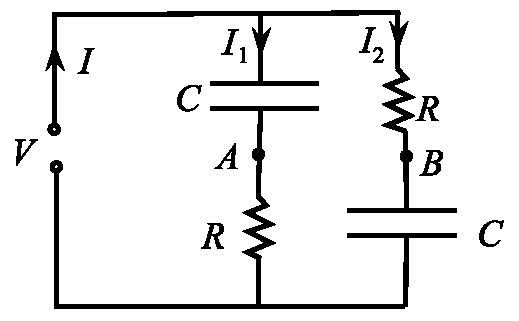
\includegraphics[width = 5cm]{Purcell812}
    \caption{Circuit with resistors and capacitors }}
    \label{RCRC}
  \end{figure}
Considering the two circuit loops that contain $V_0$, we can find
the following equations relating the currents $I_1$ and $I_2$ to the voltage
$V_0$:
$$ V_0 = I_1 Z_1 = I_1\left( (\frac{-i}{\omega C}) + R\right) \qquad V_0 = I_2 Z_2  = I_2\left(R + (\frac{-i}{\omega C})\right)$$
The voltage $V_{AB} = V_B - V_A$ is then:
$$V_{AB} = -I_2 R + I_1( \frac{-i}{\omega C})$$
Substituting for the currents $I_1$ and $I_2$, we find:
$$V_{AB} = -\frac{V_0 R}{R +( \frac{-i}{\omega C})} + \frac{V_0( \frac{-i}{\omega C})}{R + (\frac{-i}{\omega
C})} = -V_0\frac{R + \frac{i}{\omega C}}{R - \frac{i}{\omega C}} =
V_0\frac{1 - i \omega RC}{1 + i \omega RC}$$
We can take the absolute value of both side to get:
$$|V_{AB}|^2 = |V_0|^2\left(\frac{1-i\omega RC}{1+i\omega RC}\right)\left(\frac{1+i\omega RC}{1-i\omega
RC}\right) = |V_0|^2\frac{1 + (RC\omega)^2}{1 + (RC\omega)^2} =
|V_0|^2$$
In order for $V_{AB}$ and $V_0$ to be out of phase by $\phi =
-{\pi}/{2}$, we must have $$V_{AB} = V_0e^{i\phi} =
V_0e^{-i\frac{\pi}{2}} = -iV_0$$ Therefore ,
$$\frac{1 - i \omega RC}{1 + i \omega RC} = -i \quad \implies
\quad \frac{1- (RC\omega)^2}{1+ (RC\omega)^2} -
i\frac{2RC\omega}{1+ (RC\omega)^2} =-i$$
Equating the real parts (the imaginary parts give the same result),
we find:
$$1-(RC\omega)^2 = 0  \quad \implies \quad \omega =
\frac{1}{RC}$$


\end{solution}



\begin{problem}{Purcell 8.16}


\begin{figure}[H]
    \centering
    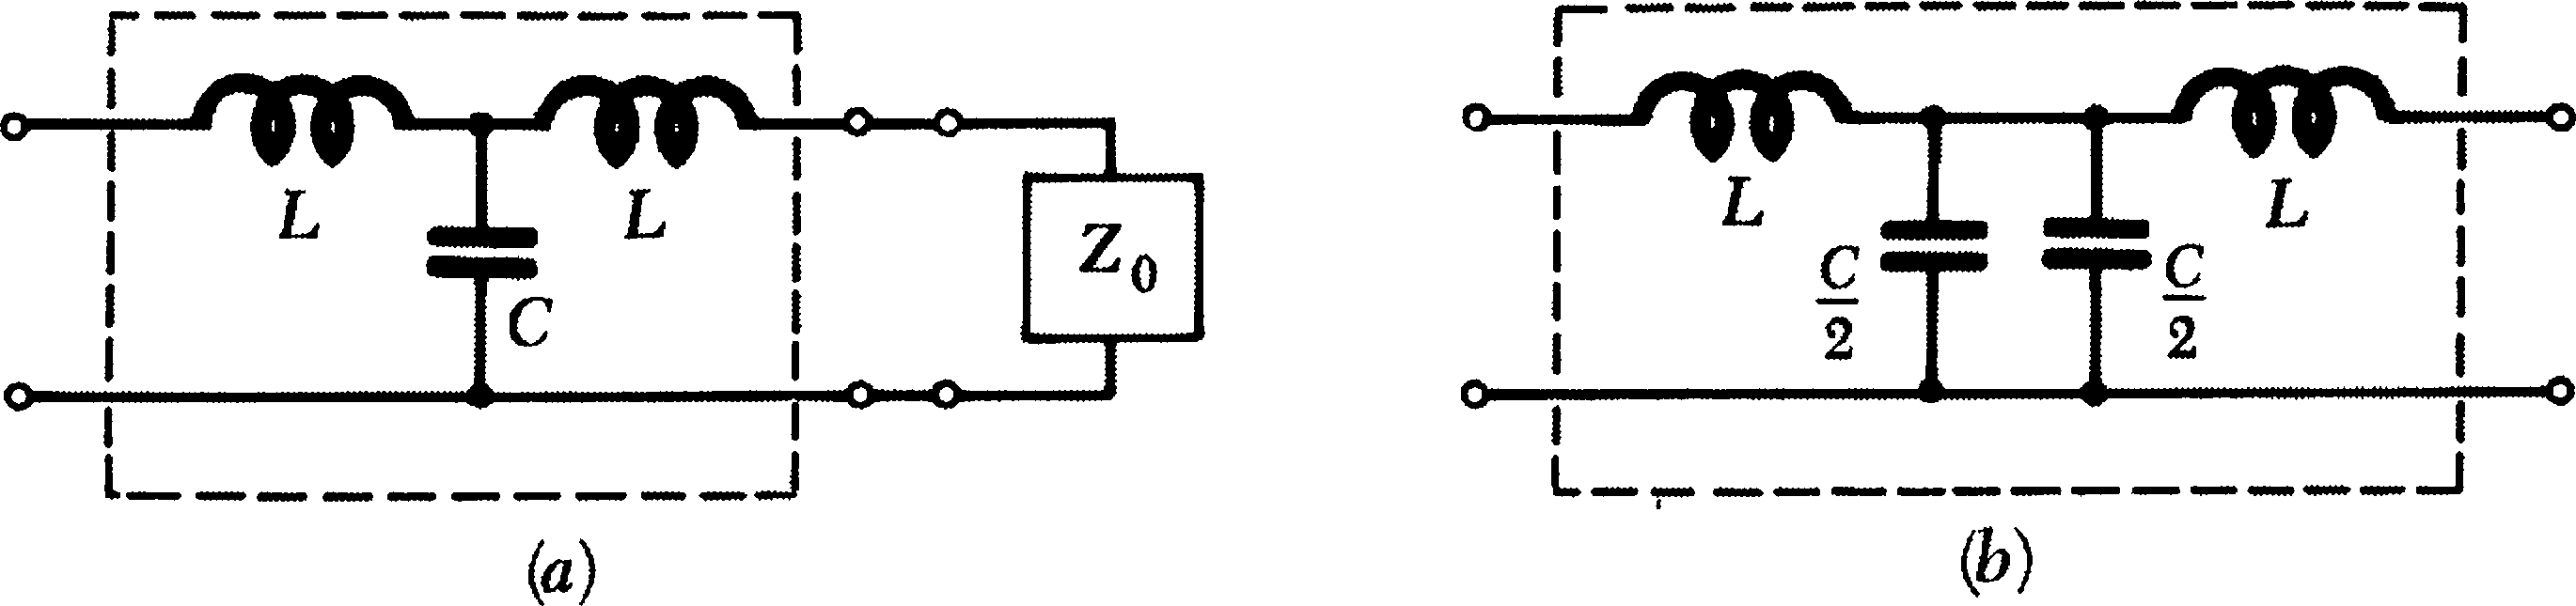
\includegraphics[width = 10cm]{pu816}
    \caption{Purcell 8.16}}
    \label{pu816}
  \end{figure}

An impedance $Z_o$ is to be connected to the terminals on the right. For given frequency $\omega$ find the value which $Z_o$ must have if the resulting impedance between the left terminals is $Z_o$. The required $Z_o$ is a pure resistance $R_o$ provided $\omega^2<2/LC$. What is $Z_o$ in the special case $\omega = \sqrt{2/LC}$?


\end{problem}



\begin{solution}
We combine the impedances like resistances so that the total impedance is
\[ Z = Z_L + \frac{1}{\frac{1}{Z_C} + \frac{1}{Z_L + Z_o}}\ \ , \]
with $Z_L = i\omega L$ and $Z_C = 1/i\omega C$. We set this equal to $Z_o$ and simplify to obtain
\[ Z_o = \sqrt{-\omega^2L^2 + 2L/C}\ \ .\]
This will be pure real and thus a pure resistance if
\[ -\omega^2L^2 + 2\frac{L}{C} >0 \ \ ,\]
\[ \omega^2 < \frac{2}{LC}\ \ .\]
In the special case $\omega = \sqrt{2/LC}$, we have $Z_o=0$. 
\end{solution}

\begin{problem}{Optional Purcell 8.10}
\begin{figure}[H]
    \centering
    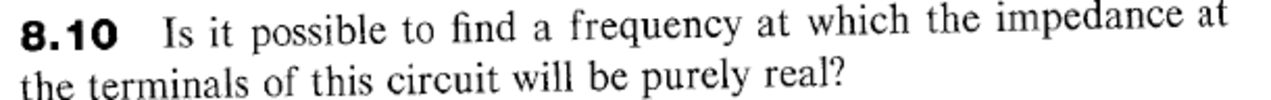
\includegraphics[width = 10cm]{pu810}
    \caption{Purcell 8.10}
  \end{figure}
  
  \begin{figure}[H]
    \centering
    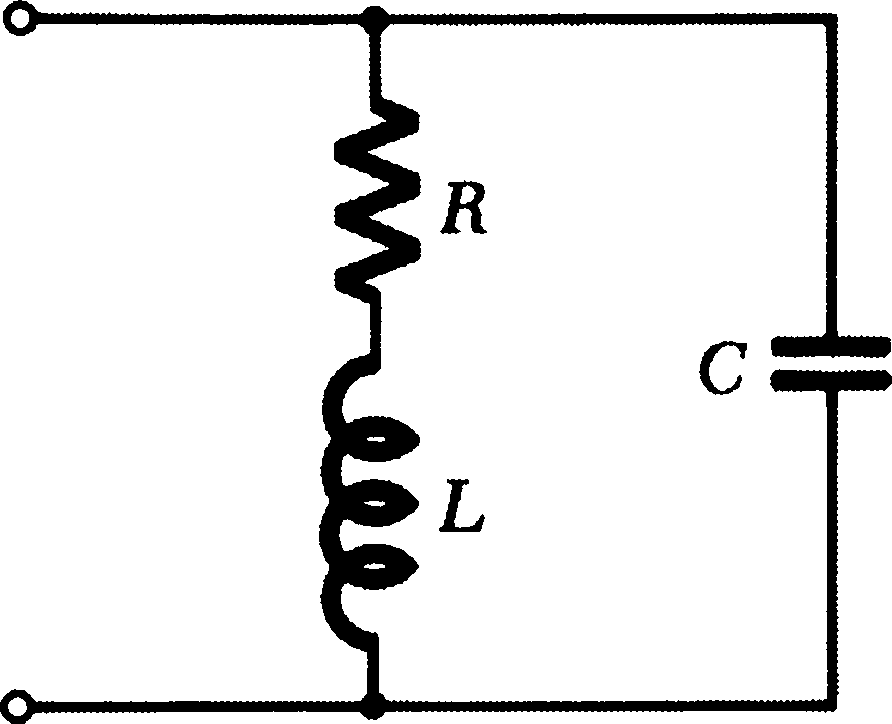
\includegraphics[width = 10cm]{figpu810}
    \caption{Purcell 8.10}
  \end{figure}
\end{problem}
\begin{solution}
\begin{eqnarray}
\frac{1}{Z} &=& i\omega C + \frac{1}{R+i\omega L}\nonumber\\
\frac{1}{Z} &=&\left[i\omega C+\frac{R-i\omega L}{R^2+(\omega
L)^2}\right]\nonumber\\
&=& \left[ i(\omega C-\frac{\omega L}{R^2+(\omega
L)^2})+(\textrm{real part})\right].
\end{eqnarray}
To make Z purely real, $Z^{-1}$ must be real.  So
\begin{eqnarray}
\omega C &=& \frac{\omega L}{R^2+(\omega L)^2},\\
\omega &=& \sqrt{\frac{L-CR^2}{CL^2}}.
\end{eqnarray}

Noth that the argument inside a square root must be positive.
Therefore the condition under which it is possible to find 
a frequency so that $Z$ is purely real is 
\begin{equation}
L/C>R^2.
\end{equation}
\end{solution}


\begin{problem}{ Optional Purcell 8.13}

\begin{figure}[H]
    \centering
    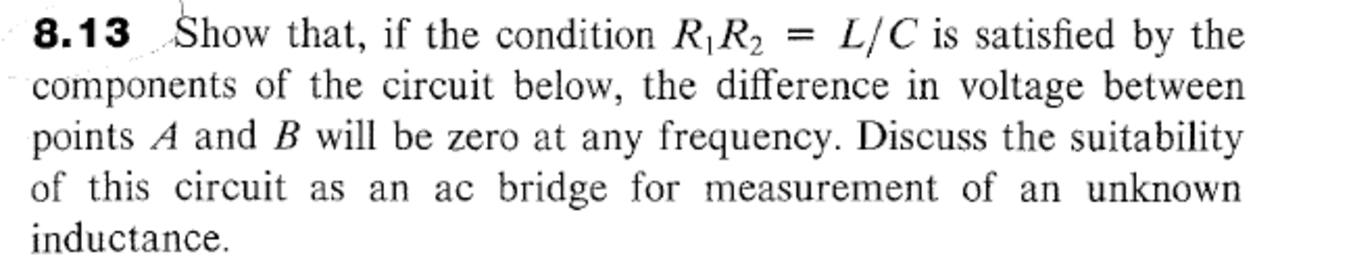
\includegraphics[width = 10cm]{pu813}
    \caption{Purcell 8.13}
  \end{figure}
  
  \begin{figure}[H]
    \centering
    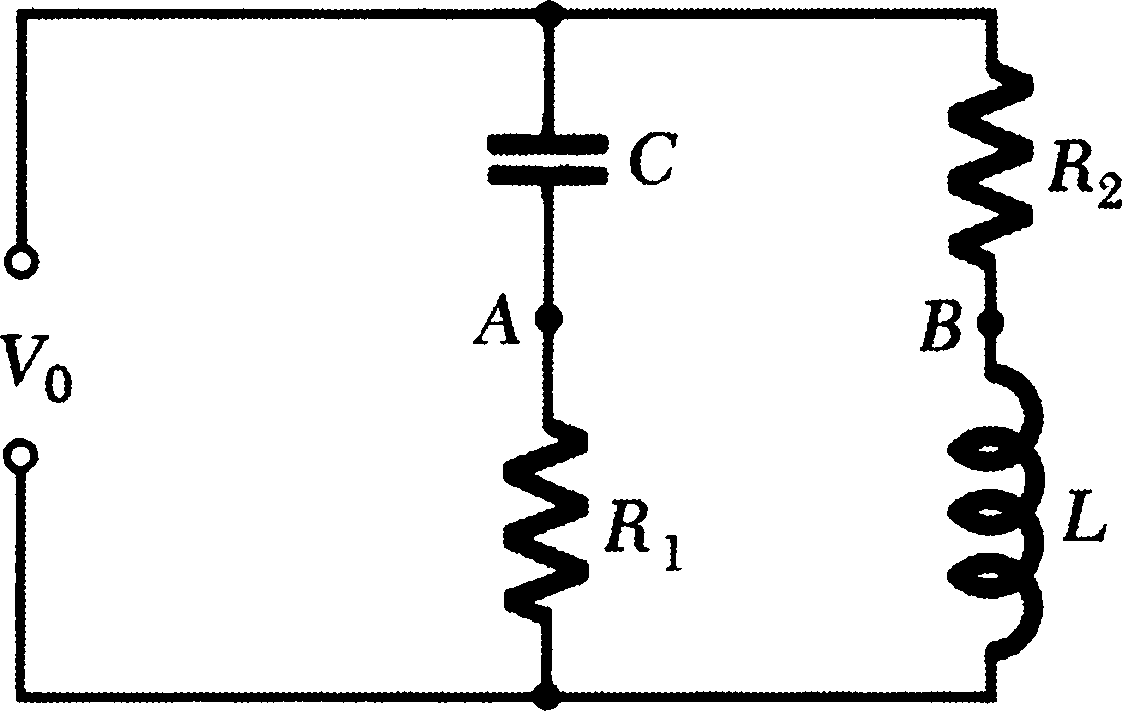
\includegraphics[width = 10cm]{figpu813}
    \caption{Purcell 8.13}
  \end{figure}

\end{problem}
\begin{solution}
Refer to the figure for Problem 8.13 of Purcell p.321.  The impedance
of the left path ($C-R_1$) and the right ($R_2 - L$) are respectively
\[Z_1=R_1-\frac{i}{\omega C},\;\;\;\;\;\; Z_2=R_2+i\omega L.\]
Set the voltage at the bottom of the circuit to be zero.  Then the
voltages at the points A and B are respectively
\begin{eqnarray}
V_A &=& \frac{V_0}{Z_1} R_1= \frac{V_0 R_1}{R_1-\frac{i}{\omega
C}},\nonumber\\
V_B &=& \frac{V_0}{Z_2} (i\omega L)=\frac{V_0 i\omega L}{R_2+i\omega L}.
\end{eqnarray}
Solve $V_A=V_B$.
\begin{eqnarray}
R_1(R_2+i\omega L) &=& i\omega L (R_1-\frac{i}{\omega C})\nonumber\\
\textrm{or}\qquad\qquad R_1 R_2 &=& L/C.\label{eqn5:condition}
\end{eqnarray}

Since condition (\ref{eqn5:condition}) doesn't depend on the value of
frequency, we conclude that, if condition (\ref{eqn5:condition}) is
satisfied, the voltage difference between points A and B will be zero
at any frequency.\\

We may employ this condition to measure unknown inductance.  The
circuit is exactly the same, but we connect points A and B by an AC
voltmeter.  The values of $R_1$, $R_2$ and $C$ are known; at least one
of the resistance should be adjustable.  We then adjust the resistance
so that the reading in the voltmeter vanishes.  If necessary, we may
adjust the frequency to check that this vanishing doesn't depend on
frequency.  At the vanishing point the condition
(\ref{eqn5:condition}) is satisfied and the inductance is measured by
$L=R_1 R_2 C$.

\end{solution}

\begin{problem}{Optional Purcell 8.14}
\begin{figure}[H]
    \centering
    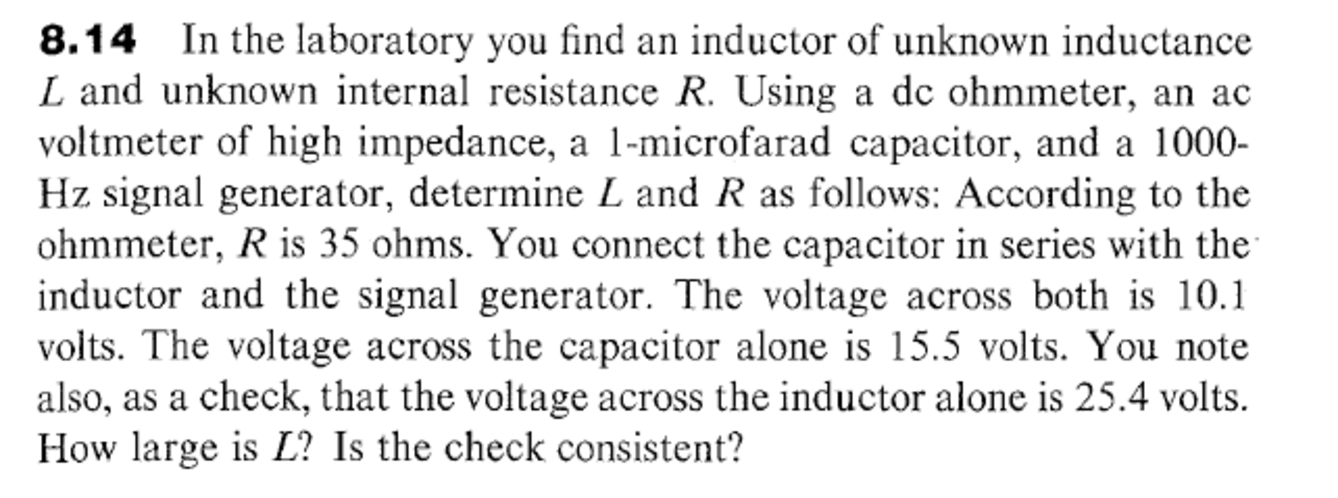
\includegraphics[width = 10cm]{pu814}
    \caption{Purcell 8.14}
  \end{figure}
  
  
\end{problem}
\begin{solution}
Consider the RLC in series.  
\begin{equation}
Z_{LR}=R+i\omega L\,,\qquad Z_c=-i/\omega C\,,\qquad
Z_{\textrm{total}}=R+i(\omega L-1/\omega C)\,.
\end{equation}

From the potential across both and across the capacitor,
\begin{eqnarray}
\frac{V_{\textrm{total}}}{V_C}&=&\frac{Z_{\textrm{total}}}{Z_C}=i\omega
CR+(1-\omega^2 CL)\,,\\
\textrm{so}\qquad \left| \frac{V_{\textrm{total}}}{V_C}\right| &=&
\sqrt{(\omega CR)^2+(1-\omega^2 CL)^2}\,,
\end{eqnarray}

After doing some math, we find the expression for L,
\begin{equation}
\qquad L = \frac{1}{\omega^2 C}\left[
1\pm \sqrt{\left|\frac{V_{\textrm{total}}}{V_C}\right|^2-(\omega CR)^2}
\right]
\end{equation}

Plug in $\omega=2\pi f=2\pi\times 1000\textrm{ Hz}$,
$V_{\textrm{total}}=10.1\textrm{ volts}$, $V_C=15.5\textrm{ volts}$,
$C=10^{-6}\textrm{ farad}$, $R=35\textrm{ ohm}$, we get 
\[ L= 0.041 \textrm{ henry}\qquad\textrm{or}\qquad 0.0098\textrm{ henry}.\]

To check the consistency, calculate the ratio
\begin{eqnarray}
\frac{V_{LR}}{V_C}&=&\frac{Z_{LR}}{Z_C}=i\omega CR-\omega^2 CL\\
\textrm{so}\qquad \left|\frac{V_{LR}}{V_C}\right| &=& \sqrt{(\omega
CR)^2+(\omega^2 CL)^2}\\
&=& 1.63 \textrm{ for L=0.041 henry}\nonumber\\
& & 0.45\textrm{ for L=0.0098 henry}.
\end{eqnarray}

The measurement gives $\left|\frac{V_{LR}}{V_C}\right| =
25.4/15.5=1.64$.  So the correct value for L is L=0.041 henry and the
check is consistent.
\end{solution}

\end{document}
